\subsection{Subclass}
\begin{itemize}
	\item In Flatland, soldiers and craftsmen have something in common: they are both workers, represented by triangles.
	\item We can represent this kind of relationship between two C++ classes with a \textit{derived class} (or referred to as: \textit{inherited class} or \textit{subclass})
	\item Subclasses contain all of the functionality and data of their parent class
	\item An ``is a'' relationship
	\item e.g.,
\begin{lstlisting}[style=C++]
class Isosceles: public Triangle {
	// ...
}
\end{lstlisting}
	\item Isosceles ``is a'' triangle
\end{itemize}

\subsection{Class hierarchy}
\begin{itemize}
	\item Derivation is often represented by a graph, where each vertex is a class, and each edge shows derivation
	\begin{center}
		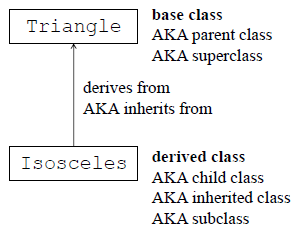
\includegraphics{sections/lec11/hi.png}
	\end{center}
\end{itemize}

\subsection{Adding member functions}
\begin{itemize}
	\item Subclasses need to respect the abstraction of their parent classes
	\item Use getters and setters to deal with private variables
\end{itemize}

\subsection{Derived class constructors}
\begin{itemize}
	\item Constructors \textbf{are not} inherited.
	\item Constructors run automatically, \textbf{starting with the base class}.
	\item e.g.,
	\begin{itemize}
		\item First, \lstinline[style=C++]{Triangle} constructor runs
		\item Then, \lstinline[style=C++]{Isosceles} constructor runs
	\end{itemize}
	\item You can also re-use the parent class constructor:
\begin{lstlisting}[style=C++]
Isosceles(double base, double leg): Triangle (base, leg, leg) {}
\end{lstlisting}
	\item But do not call the parent constructor outside the initializer list
	\item \textbf{DO NOT DO THIS:}
\begin{lstlisting}[style=C++]
Isosceles(double base, double leg){
	Triangle(base, leg, leg); // BAD - anonymous object
}
\end{lstlisting}
\end{itemize}

\subsection{Override vs. Overload}
\begin{itemize}
	\item A function \textbf{override} is where a derived class has a function with the same name and prototype as the parent
\begin{lstlisting}[style=C++]
Triangle::set_b(double b_in);
Isosceles::set_b(double b_in);
\end{lstlisting}
	\item A function \textbf{overload} is where a single class has two different functions with the same name, but different prototypes
\begin{lstlisting}[style=C++]
Triangle::Triangle();
Triangle::Triangle(double a_in,double b_in,double c_in);
\end{lstlisting}
\end{itemize}

\subsection{protected members}
\begin{itemize}
	\item \lstinline[style=C++]{protected} members can be seen by all members of this class and any derived classes
\begin{lstlisting}[style=C++]
class Triangle {
public:
	//member functions ...
protected:
	//edge lengths represent a triangle
	double a,b,c;
};
\end{lstlisting}
	\item Use the scope resolution operator (::) to call inherited functions: \lstinline[style=C++]{Triangle::set_b(b_in);}
\end{itemize}

\subsection{Liskov Substitution Principle}
\begin{itemize}
	\item If S is a subtypeof T, then objects of type T may be replaced with objects of type S without altering any of the desirable properties of that program (correctness)
	\item Or: For any instance where an object of type T is expected, an object of type S can be supplied without changing the correctness of the original computation
	\item Not all C++ derived classes are subtypes
	\item For a derived type to also be a subtype, code written to correctly use the supertypemust still be correct if it uses the subtype
	\item 
\end{itemize}

\subsection{How to create a subtype}
\begin{itemize}
	\item With Abstract Data Types, there are three ways to create a subtype from a derived type:
	\begin{enumerate}
		\item Weaken the precondition of one or more operations
		\item Strengthen the postconditionof one or more operations
		\item Add one or more operations
	\end{enumerate}
	\item 1 \& 2 apply to overriden functions:
	\begin{itemize}
		\item The overridden member function must require no more of the caller than the old method did, but it can require less
		\item The overridden member function must do everything the old function did, but it is allowed to do more as well
	\end{itemize}
\end{itemize}

\subsubsection{Weaken precondition}
\begin{itemize}
	\item The preconditions of a method are formed by two things:
	\begin{itemize}
		\item Its argument type signature
		\item The REQUIRES clause
	\end{itemize}
	\item We can weaken the preconditions by requiring less:
\begin{lstlisting}[style=C++]
//REQUIRES: b_inis non-negative and forms a
// triangle with existing edges
//MODIFIES: this
//EFFECTS: sets edges b and c
void Isosceles::set_b(double b_in) {
	Triangle::set_b(b_in);
	Triangle::set_c(b_in);
}

//Becomes:
//REQUIRES: b_inis non-negative andforms a
// triangle with existing edges
//MODIFIES: this
//EFFECTS: sets edges b and c
void Isosceles::set_b(double b_in) {
	b_in= abs(b_in);
	Triangle::set_b(b_in);
	Triangle::set_c(b_in);
}
\end{lstlisting}
\end{itemize}

\subsubsection{Strengthen postcondition}
\begin{itemize}
	\item The postconditionsof a method are formed by two things:
	\begin{itemize}
		\item Its return type signature
		\item The EFFECTS clause
	\end{itemize}
	\item We can strengthen the EFFECTS clause by promising everything we used to, plus extra
\begin{lstlisting}[style=C++]
void Isosceles::set_b(double b_in) {
	Triangle::set_b(b_in); //does everything Triangle did
	Triangle::set_c(b_in); //plus more
}
\end{lstlisting}
\end{itemize}

\subsubsection{Add an operation}
\begin{itemize}
	\item The final way of creating a subtype is to add a member function
	\item Any code expecting only the old function will still see all of them, so the new function won't break old code
\begin{lstlisting}[style=C++]
class Isosceles : public Triangle {
public:
	//...
	void set_base(double base){/*...*/}
	void set_leg(double leg) {/*...*/}
};
\end{lstlisting}
\end{itemize}